\setAuthor{Richard Luhtaru}
\setRound{lõppvoor}
\setYear{2024}
\setNumber{G 4}
\setDifficulty{4}
\setTopic{TODO}

\prob{Piljard}
Piljardikuul massiga $m=\SI{200}{\g}$ ja algkiirusega $v_0=\SI{1}{\m\per\s}$ põrkab mitteelastselt vastu piljardilaua serva, nii et nurk enne põrget on $\ang{45}$ ja nurk pärast põrget on $\ang{60}$. Eeldage, et piljardilaua serv mõjutab kuuli ainult servaga risti olevas sihis. Leidke\\
\osa mitu protsenti piljardikuuli energiast läks põrke jooksul kaduma;\\
\osa kui suur oli keskmine põrke jooksul kuulile mõjuv jõud $F_p$, eeldades, et põrge kestis $t_p=\SI{0.01}{\s}$.
\begin{center}
  \vspace{-1em}
  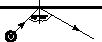
\includegraphics[width=0.6\linewidth]{2024-v3g-04-yl.pdf}
  \vspace{-1em}
\end{center}



\hint

\solu
\par
\osa Olgu piljardikuuli kiirus enne põrget $v_0$ ja pärast põrget $v_1$. Olgu $x$-telg servaga paralleelne ja $y$-telg servaga risti. Kuna serv mõjutab kuuli ainult $y$-sihis, siis kuuli $x$-suunaline kiirus ei muutu põrke jooksul. Seega
\begin{equation*}
    v_x = v_0\sin\ang{45} = v_1\sin\ang{60} \implies \frac{v_1}{v_0} = \frac{\sin\ang{45}}{\sin\ang{60}}.
\end{equation*}
Kuna kuuli kineetiline energia on $E = \frac{1}{2}mv^2$, siis
\begin{equation*}
    \frac{E_1}{E_0} = \frac{\frac{1}{2}mv_1^2}{\frac{1}{2}mv_0^2} = \frac{v_1^2}{v_0^2} = \frac{\sin^2\ang{45}}{\sin^2\ang{60}} = \left(\frac{\sqrt{2}/2}{\sqrt{3}/2}\right)^2 = \frac{2}{3},
\end{equation*}
seega põrke käigus läks kaduma umbes $33\%$ palli energiast.

\osa Newtoni teisest seadusest
\begin{equation*}
    F = ma = m\frac{\Delta v}{\Delta t} \implies F\Delta t = m\Delta v.
\end{equation*}
Kuna jõud mõjus kuulile ainult $y$-suunas, siis järelikult
\begin{equation*}
    F_p t_p = m\left(v_{1,y}-v_{0,y}\right)
\end{equation*}
(kus loeme $v_y$ positiivseks, kui kiirus on suunatud lauast eemale). Me teame, et
\begin{align*}
    v_{0,y} &= -v_0 \cos\ang{45} = -\frac{\sqrt 2}{2}v_0,\\
    v_{1,y} &= v_1 \cos\ang{60} = \sqrt{\frac{2}{3}}v_0\cos\ang{60} = \frac{\sqrt 2}{2\sqrt 3}v_0,
\end{align*}
seega
\begin{equation*}
    \Delta v_y = v_{1,y}-v_{0,y} = \left(\frac{\sqrt 2}{2\sqrt 3} + \frac{\sqrt 2}{2}\right)v_0 \approx \SI{1.115}{\m\per\s}.
\end{equation*}
Keskmine kuulile mõjuv jõud oli järelikult
\begin{equation*}
    F_p = \frac{m\Delta v_y}{t_p} = \frac{\SI{0.2}{\kg}\cdot \SI{1.115}{\m\per\s}}{\SI{0.01}{\s}} = \SI{22.3}{N}.
\end{equation*}
\probend